%!TEX root = pset3.tex

\section{Neural Networks}\label{sec:neural_networks}

Neural networks are used in machine learning to make predictions, similar to logistic regression, SVM, or regression.  We can represent neural networks using a graph with nodes and edges (see Bishop figure 5.1).  Assume that we observe data $(\M{x}^{(n)},\M{y}^{(n)}), n = 1, \ldots, N$,  where $\M{x}^{(n)} \in \mathbb{R}^{D+1}$ (including the bias term) and $\M{y}^{(n)} \in \{0,1\}^K$.  Let $(\M{x},\M{y}) = ([x_0, x_1, \ldots, x_D],[y_1, \ldots, y_K])$ be a general observation, where $x_0 = 1$ is a constant term for the bias.  In this example, only one term of $[y_1, \ldots, y_K])$ can be one; the rest are zero. We create nodes for each of the features $x_i$, referred to as \emph{inputs}, and nodes for each of the class labels $y_i$, referred to as \emph{outputs}.  Next, we introduce a series of nodes in the middle of the graph, called \emph{hidden units}, and we draw edges connecting the {\bf inputs} $\rightarrow ${\bf hidden units}$ \rightarrow$ \emph{\bf outputs}.  The key idea in neural networks is that we can model the hidden units as functions of the inputs, and model the outputs as functions of the hidden units.   

For 2-layer neural networks, we have one layer of hidden units denoted by $[z_0, z_1,\ldots, z_M]$.   There are weights $\M{w}^{(1)}_{ji}$ for each edge $x_i \rightarrow z_j$ and $\M{w}^{(2)}_{kj}$ for each edge $z_j \rightarrow y_k$, which are unknown and will be learned through training the model.  However, there are no edges from the inputs to $z_0$, because we assume $z_0 = 1$ is a constant term for the bias.  Let $\sigma(\cdot)$ denote the logistic function, which we will use as the \emph{activation function} for both the hidden and output layers of our neural network.  The predicted value for output $k$ given parameters $\M{w} = (\M{w}^{(1)}, \M{w}^{(2)})$ and input $\M{x}$ will be:

\begin{equation}
h_{k}(\M{x},\M{w}) = \sigma\left(\sum_{j=1}^{M} w^{(2)}_{kj} \sigma\left(\sum_{i=0}^{D} w^{(1)}_{ji} x_i\right)  + w_{k0}^{(2)} \right).
\end{equation}

\subsection{Implementation}

\subsubsection{Gradient Descent}
We implemented a 2-layer regularized neural network using gradient descent.  The loss function, which is the negative log-likelihood, is equal to:
\begin{equation}
\ell(\M{w}) \equiv \sum_{n=1}^{N} \sum_{k=1}^{K} \left[ -y_k^{(n)} \log(h_{k}(\M{x}^{(n)}, \M{w})) - (1-y_k^{(n)}) \log(1 - h_{k}(\M{x}^{(n)}, \M{w}))\right]
\end{equation}

Let $\M{\tilde w}^{(1)} = (\M{w}^{(1)}_{ji})_{i \neq 0}$ and $\M{\tilde w}^{(2)} = (\M{w}^{(2)}_{kj})_{j \neq 0}$. We add a regularizer term, and the final cost function becomes:
\begin{equation}
J(\M{w}) \equiv \ell(\M{w}) + \lambda(\|\M{\tilde w}^{(1)}\|^2_F + \|\M{\tilde w}^{(2)}\|^2_F),
\end{equation}

where $\|A\|_F = \sqrt{\sum_{i,j} A^2_{ij}}$ is the matrix Frobenius norm, and $\lambda$ is a fixed parameter chosen via cross-validation.  Note that we exclude the bias terms from our regularizer in order to avoid penalty if the data is shifted.  To take the derivative of this function, we introduce some more notation:

\begin{equation}
a^{(1)}_j(\M{x}) \equiv \sum_{i=0}^D w_{ji}^{(1)} x_i
\end{equation}
\begin{equation}
z_j(\M{x}) \equiv \left\{\begin{array}{rl}
\sigma(a^{(1)}_j(\M{x})), & ~~~ j = 1,\ldots, M\\
1, & ~~~j = 0 \end{array} \right.
\end{equation}
\begin{equation}
a^{(2)}_k(\M{x}) \equiv \sum_{j=0}^M w_{kj}^{(2)} z_j(\M{x})
\end{equation}

We refer to $a^{(1)}_j(\M{x})$ and $a^{(2)}_k(\M{x})$ as the \emph{activations} for a fixed value of $\M{x}$.  It follows that $h_{k}(\M{x},\M{w}) = \sigma(a^{(2)}_k(\M{x}))$. Taking partial derivatives of $J$ with respect to $\M{w}^{(2)}_{kj}$ and $\M{w}^{(1)}_{ji}$ for $i \neq 0$ and $j \neq 0$, we find:  

\begin{align}
\frac{\partial J(\M{w})}{\partial \M{w}^{(2)}_{kj}} &= 2 \lambda \M{w}^{(2)}_{kj} + \frac{1}{N}\sum_{n=1}^{N} \left(\frac{-y_k^{(n)}}{h_k(\M{x}^{(n)},\M{w})} +  \frac{1-y_k^{(n)}}{1 - h_k(\M{x}^{(n)},\M{w})}\right) h_k(\M{x}^{(n)},\M{w}) (1 - h_k(\M{x}^{(n)},\M{w})) z_j(\M{x}^{(n)})\\
&= 2 \lambda \M{w}^{(2)}_{kj} +  \frac{1}{N}\sum_{n=1}^{N} \left(-y_k^{(n)}(1 - h_k(\M{x}^{(n)},\M{w})) + (1-y_k^{(n)})h_k(\M{x}^{(n)},\M{w}) \right) z_j(\M{x}^{(n)})
\end{align}

\begin{equation}
\frac{\partial J(\M{w})}{\partial \M{w}^{(1)}_{ji}} =  2 \lambda \M{w}^{(1)}_{ji}  + \frac{1}{N}\sum_{n=1}^{N} \sum_{k=1}^{K} \left(-y_k^{(n)}(1 - h_k(\M{x}^{(n)},\M{w})) + (1-y_k^{(n)})h_k(\M{x}^{(n)},\M{w}) \right)w_{kj}^{(2)} z_j(\M{x}^{(n)})(1-z_j(\M{x}^{(n)})) \M x^{(n)}
\end{equation}

For the bias terms, there is no regularizer penalty, so we obtain:
\begin{equation}
\frac{\partial J(\M{w})}{\partial \M{w}^{(2)}_{k0}} = \frac{1}{N}\sum_{n=1}^{N} \left(-y_k^{(n)}(1 - h_k(\M{x}^{(n)},\M{w})) + (1-y_k^{(n)})h_k(\M{x}^{(n)},\M{w}) \right)
\end{equation}
\begin{equation}
\frac{\partial J(\M{w})}{\partial \M{w}^{(1)}_{j0}} =  \frac{1}{N} \sum_{n=1}^{N} \sum_{k=1}^{K} \left(-y_k^{(n)}(1 - h_k(\M{x}^{(n)},\M{w})) + (1-y_k^{(n)})h_k(\M{x}^{(n)},\M{w}) \right)w_{kj}^{(2)} z_j(\M{x}^{(n)})(1-z_j(\M{x}^{(n)})) \M x^{(n)}
\end{equation}

Therefore, we have calculated analytic expressions for the gradients of $J$ with respect to the different groups of parameters $\M{w}^{(2)}$ and $\M{w}^{(1)}$.  From these expressions, we coded a function in MATLAB to train a our neural network using \textit{batch gradient descent}. The function takes in all the input data $(\M{x}^{(n)},\M{y}^{(n)}), n = 1, \ldots, N$ at once, and does gradient descent on the total objective value over the $N$ data points each time, until convergence. Model parameters are regularization parameter $\lambda$, number of nodes in the hidden layer $M$, and initial solution $(\M{w}^{(1)}_{init}, \M{w}^{(2)}_{init})$. The function outputs the optimal solution $\M{w} = (\M{w}^{(1)}, \M{w}^{(2)})$ that minimizes the final cost function $J(\M{w})$. The formula for the update is as follows:

\begin{equation}
\M w^{(1)}_{new} = \M w^{(1)}_{old} - \eta \nabla_{w^{(1)}}J(\M w_{old}),~~~~~~\\
\M w^{(2)}_{new} = \M w^{(2)}_{old} - \eta \nabla_{w^{(2)}}J(\M w_{old})
\end{equation}


Because the objective function is non-convex, we run our training function with multiple initial solutions to avoid reporting a single local optimum.  After running multiple times, we report the optimal solution $\M{w} = (\M{w}^{(1)}, \M{w}^{(2)})$ that minimizes $J(\M{w})$ over all trials. % The gradient descent function used 

\subsubsection{Stochastic Gradient Descent}

We implemented an alternate function in MATLAB to train our neural network using \textit{stochastic gradient descent}. We first take one training point and run gradient descent on the objective function on this point. With the output $\M{w}^{(1)}$ and $\M{w}^{(2)}$ as new initial values, we then take a second point and run gradient descent on the objective function on this point. Repeat the process until convergence. If necessary, we can reshuffle the data and loop through the data multiple times.


\subsection{Computational Results}

We tested our neural network on various data sets, including toy problems and real-world MNIST data on hand-written digits. Both batch gradient descent and stochastic gradient descent methods are tested on the sets. 


\subsubsection{Toy Problems}

The first toy problem is on a linearly separable 3-class data. The decision boundary of a good ANN classifier we found is illustrated in Figure~\ref{fig:toy_1}. We present the validation set accuracy results in Table~\ref{tab:toy_1_cv}, under different number of units in the hidden layer and the trade-off parameter in regularization. We see from the table that we achieve highest validation accuracy under $\lambda = 0.001$ and $M = 2$. This gives us test accuracy of $99.3\%$. 


\begin{figure}[h!]
\centering
    \begin{subfigure}[b]{0.45\textwidth}
	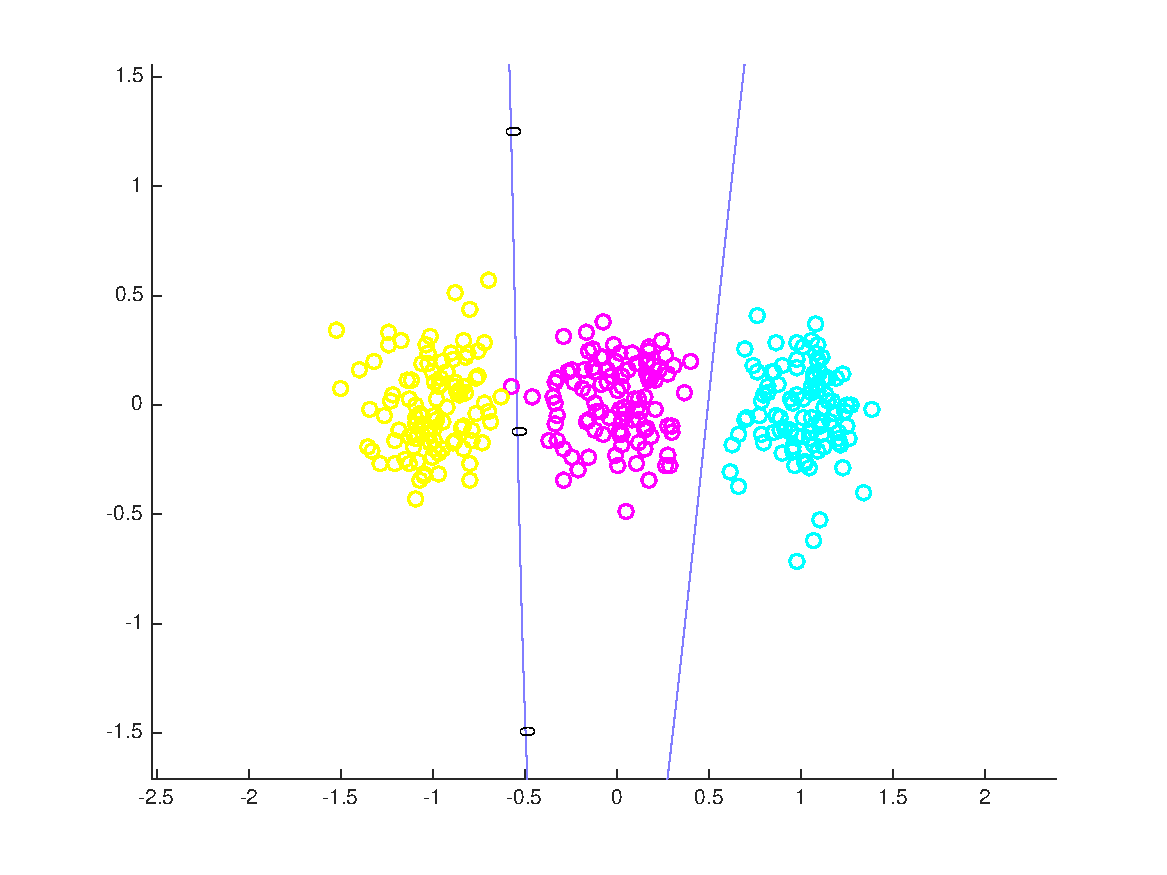
\includegraphics[height=70mm]{plot_toy_multiclass_1.pdf}
	\caption{Toy Data 1}\label{fig:toy_1}
    \end{subfigure}
    \quad
    \begin{subfigure}[b]{0.45\textwidth}
	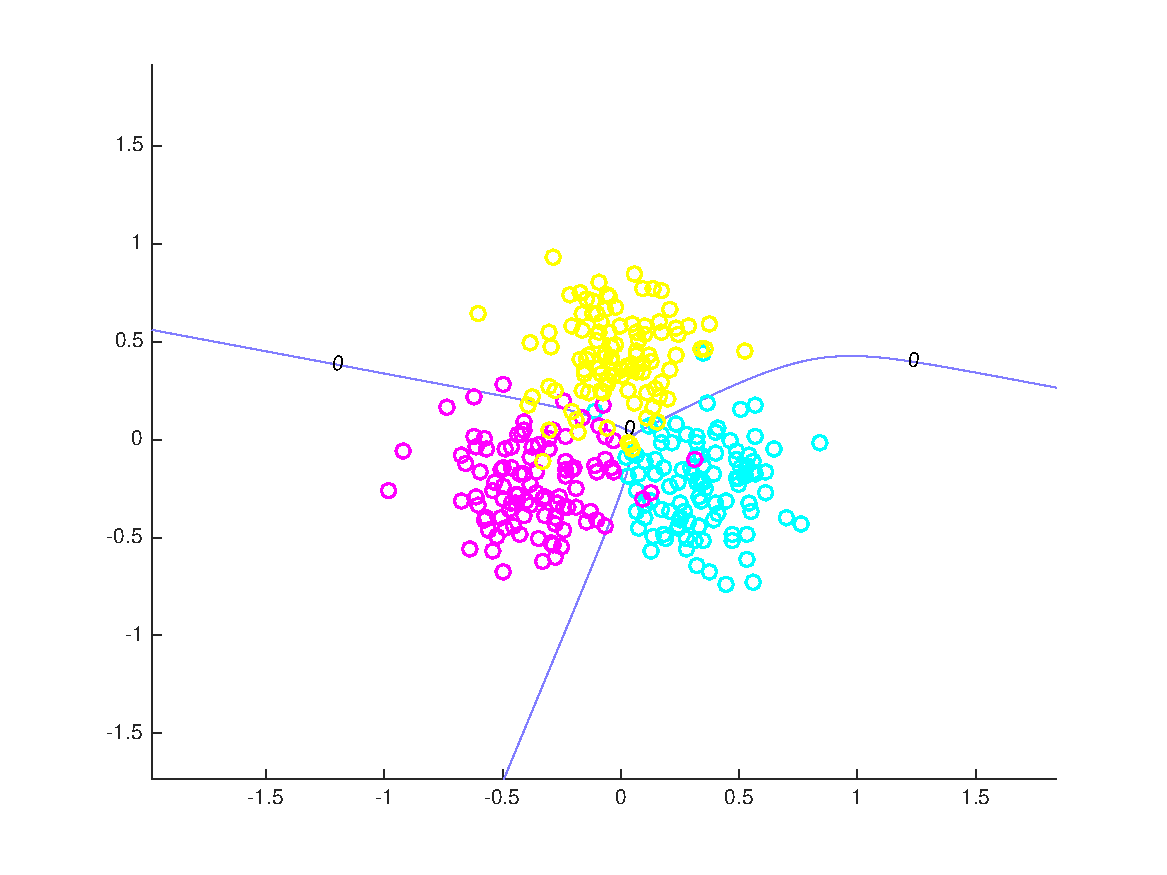
\includegraphics[height=70mm]{plot_toy_multiclass_2.pdf}
	\caption{Toy Data 2}\label{fig:toy_2}
	\end{subfigure}
    \caption{Plots of decision boundaries from Artificial Neural Networks on training toy data.}  \label{fig:LR_plots}  
\end{figure}

The second problem we considered is another 3-class data with points that are more closely spaced. The decision boundary of our ANN classifier is presented in Figure~\ref{fig:toy_2}. Similarly, the accuracy from cross-validation is given in Table~\ref{tab:toy_2_cv}. The best accuracy is obtained when $M = 4$ and $\lambda = 0.001$. This gives the testing set accuracy of $91.3\%$.


\begin{table}[h!]
\centering
\caption{Validation accuracy on Toy Data 1 under different parameter specification}\label{tab:toy_1_cv}
\begin{tabular}{ lccccc }
\hline\hline
$\lambda$ / $M$ 		& 2 		& 3			&4			&5		&6\\
\hline
0 				& 0.9933    & 0.9900    & 0.9933   &  0.9900  &   0.9933\\
0.001 			& 0.9967    & 0.9833    & 0.9867    & 0.9800   &  0.9933\\
0.01				& 0.9833    & 0.9733    & 0.9667    & 0.9833   & 0.9900\\
\hline\hline
\end{tabular}
\end{table}
         
         
\begin{table}[h!]
\centering
\caption{Validation accuracy on Toy Data 2 under different parameter specification}\label{tab:toy_2_cv}
\begin{tabular}{ lccccc }
\hline\hline
$\lambda$ / $M$ 		& 2 		& 3			&4			&5		&6\\
\hline         
0    & 0.9100    & 0.9167    & 0.9267    & 0.9167    & 0.9267\\
0.001    & 0.8967    & 0.8233    & 0.9333    & 0.9167    & 0.9333\\
0.01								& 0.8900   & 0.9233\\
\hline\hline
\end{tabular}
\end{table}


There are some computational considerations when choosing the parameters for the model. In particular, it is very important to choose reasonable initial values for $\M w$ and the step size. We chose the initial values to be a random numbers between $[-0.05, 0.05]$ because when the initial values are close to zero, the gradient on the logistic function would have a sizable magnitude. The step size is chosen to satisfy the Robbins-Monro criterion: we chose $\eta = ss/(iter + 100)^{0.6}$, where $iter$ is the number of current iteration, and $ss$ is chosen to be 25 for these toy data sets. Regarding the convergence criteria, the lower it is, the better accuracy we have generally; however the longer run-time it takes as well.

Between batch and stochastic gradient descent implementations, we found that the batch method is more sensitive to the choice of initial $\M w$. We think this might be because when doing stochastic gradient descent, some data points can pull the variables from local minimum, whereas batch gradient descent tends to get stuck somewhere more easily. The numbers we present here are from stochastic gradient descent, but can also replicated by batch method if the parameters are chosen carefully.


\subsubsection{MNIST Data}

\begin{figure}[h!]
\centering
	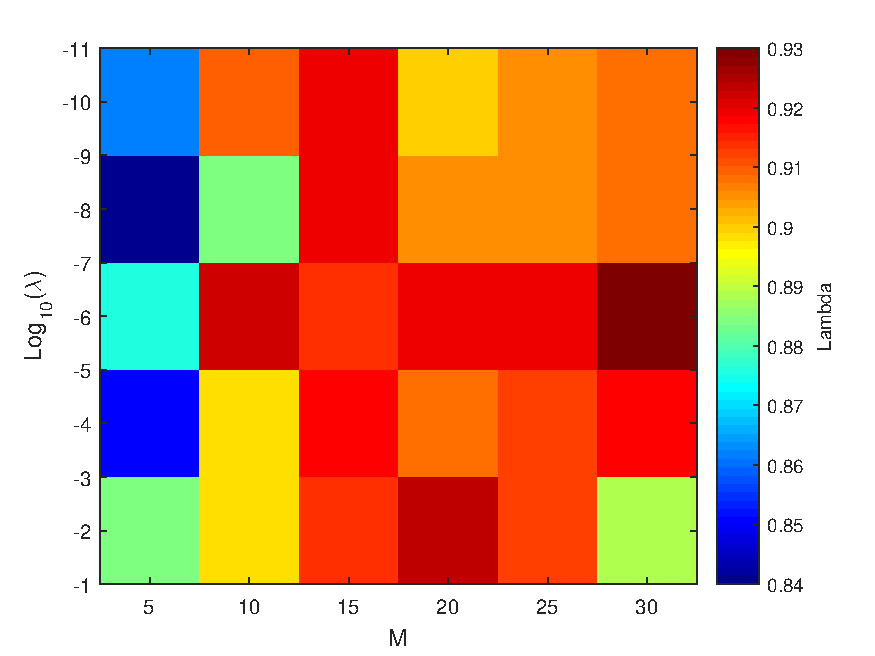
\includegraphics[height=70mm]{mnist_cv.pdf}
    \caption{Plots of decision boundaries from Artificial Neural Networks on training toy data.}  \label{fig:mnist_cv}  
\end{figure}